\chapter{The Composer and the Size Ladder}
\label{ch:composer}

\section{Composition: Definition and Verbs}

The studio's documentation refuses the word \emph{generate} for this stage, and
the reason is precision rather than pedantry: the word has been used both for the
whole pipeline and for the narrow step that turns an intent into \id{map.xml}.
There are five verbs, each meaning one thing. \textbf{Emit} fills one box with one
base shape. \textbf{Derive} reads structure back out of geometry. \textbf{Compose}
builds the plan. \textbf{Evaluate} scores a plan. \textbf{Realize} compiles a plan
into a sketch and an intent and exports it.

Emit and derive are a forward/inverse pair, and the fact that they are required to
agree is the shape model's correctness test: composition emits, verification
derives, and a disagreement is a defect in one of them.

The whole of composition is one chain, and it runs in one direction.

\begin{figure}[htbp]
\centering
\begin{tikzpicture}[
  font=\sffamily\scriptsize,
  st/.style={draw=rule, line width=0.8pt, fill=wash, rounded corners=2pt,
             minimum height=8mm, minimum width=17mm, align=center, inner sep=3pt},
  every path/.style={draw=ink60, line width=0.7pt, -{Stealth[length=3.5pt]}}
]
\node[st] (req) {request};
\node[st, right=5mm of req] (bud) {budget};
\node[st, right=5mm of bud] (all) {allocate};
\node[st, right=5mm of all] (fil) {fill};
\node[st, below=7mm of fil] (car) {carve the mid};
\node[st, left=5mm of car] (asm) {assemble};
\node[st, left=5mm of asm] (der) {derive};
\node[st, left=5mm of der] (gat) {gate};
\node[st, below=7mm of bud, fill=accentsoft!45, draw=accent!40] (plan) {plan};

\draw (req) -- (bud); \draw (bud) -- (all); \draw (all) -- (fil);
\draw (fil) -- (car); \draw (car) -- (asm); \draw (asm) -- (der); \draw (der) -- (gat);
\draw (gat) -- node[above, font=\sffamily\tiny, color=ink60] {accept} (plan);
\draw[rounded corners] (gat.south) |- ++(0,-6mm) -| node[pos=0.25, below, font=\sffamily\tiny, color=ink60] {reject: resample} (all.south);
\end{tikzpicture}
\caption{Composition. Nothing later reopens what something earlier settled, which
is what makes any property of the output traceable to the one step that fixed it.}
\label{fig:compose-chain}
\end{figure}

Two commitments shape everything downstream. Generation runs \textbf{from the hub
outward} in a relative frame and embeds into world coordinates late, so every box
but the hub is positioned against its neighbour rather than against the map. And
composition is \textbf{allocate-then-fill}: every footprint is placed before any
terrain exists, and filling never grows a box outward to accommodate what is being
put in it.

\section{Player Count and the Size Bands}

The composer takes five inputs (players per team, team count, symmetry, seed and
the cell scale), and only one of them drives the board's size. The player
count names a \textbf{size band}, and two counts inside one band compose to the
same budget, because in the model's view they are the same map.

\begin{table}[htbp]
\caption{The size-band ladder. Land per team is measured over 331 CTW corpus maps
carrying both a team count and a player cap; the budget in cells is that land
divided by the cell area.}
\label{tab:bands}
\small
\begin{tabular}{l r r r r r r}
\toprule
\textbf{Band} & \textbf{Players} & \textbf{Land/team} & \textbf{Land/player} &
\textbf{Maps} & \textbf{Budget} & \textbf{Unit share} \\
 & per team & blocks$^2$ & blocks$^2$ & measured & cells & cells \\
\midrule
nano  & 6--13 & 2250 & 225 & 77 & 140.6 & 126.6 \\
micro & 14--21 & 4025 & 242 & 90 & 251.6 & 226.4 \\
milli & 22--31 & 7075 & 270 & 65 & 442.2 & 398.0 \\
centi & 32+ & 8730 & 256 & 84 & 545.6 & 491.1 \\
\bottomrule
\end{tabular}
\end{table}

The striking thing about \cref{tab:bands} is the fourth column. Across a
four-times range in player count, the land each player gets barely moves: the fit
over the corpus is $\text{land} = 176 \times \text{players}^{1.12}$ with
$r = 0.83$ on log--log, which is about 250 square blocks per player at every size.
Mapmakers converged on that figure without anybody writing it down, and the studio
reads it back off their work rather than asserting it.

A count above centi's range is clamped into it, because centi is the top of the
ladder. That is a deliberate decision: there is no size band above it worth
composing for.

\subsection{The Four-Block Grid}

The plan works on a coarse cell grid, and the default cell is four blocks. The
reason is that the corridor widths the corpus actually contains have to be
expressible on it. Measured modal local thickness runs 8, 10, 14, 16 blocks up the
bands. At cell 4 the reachable widths are 4, 8, 12, 16, 20 and both ends of that
ladder land on one. At cell 5 they are 5, 10, 15, 20 and neither does.

\begin{table}[htbp]
\caption{Corridor widths by band, in blocks and in cells at the default scale.}
\label{tab:corridors}
\small
\begin{tabular}{l r r r r}
\toprule
\textbf{Band} & \textbf{Map corridor} & \textbf{in cells} &
\textbf{Wool corridor} & \textbf{in cells} \\
\midrule
nano  & 12 & 3 & 10 & 2 (floor) \\
micro & 14 & 4 & 12 & 3 \\
milli & 16 & 4 & 14 & 4 \\
centi & 16 & 4 & 14 & 4 \\
\bottomrule
\end{tabular}
\end{table}

The corpus also supplies the floor: ground narrower than eight blocks accounts for
between 1.5 and 4 percent of any map, which the model reads as the width authors
build down to and no further. The design vocabulary resting on it is simple: one
lane is a chokepoint, two the unstable middle, three multi-access.

\section{Constituents of a Composed Board}

\begin{figure}[htbp]
\centering
\begin{minipage}[c]{0.34\textwidth}
  \centering
  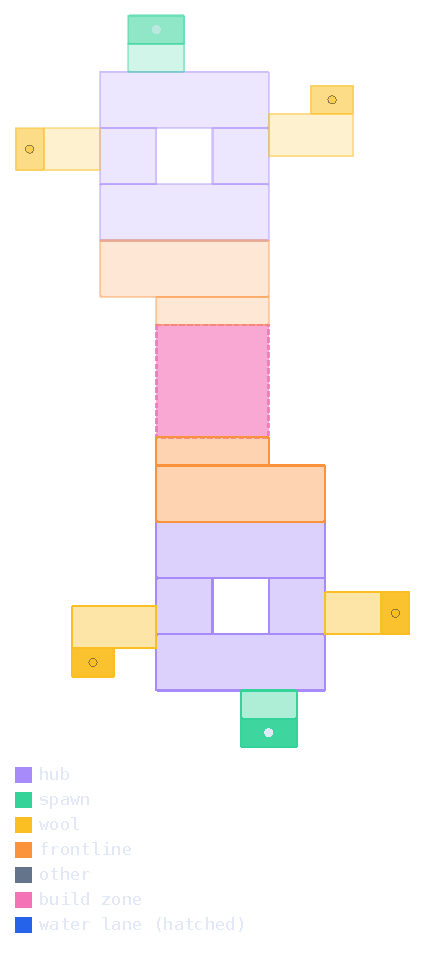
\includegraphics[height=0.52\textheight]{figures/generated/composed-hushwater.pdf}
\end{minipage}%
\hfill
\begin{minipage}[c]{0.60\textwidth}
\small
The board the worked example of \cref{ch:ctw} begins from, drawn by the studio
itself. Eighteen players a side, two teams, \id{rot\_180}, cell 4, seed 5. It
scores 0, meaning no term falls outside its band.

\medskip
Every element of \cref{tab:shares} is visible. The \textbf{hub} is the large violet
body, here in its \emph{ring} form, and the white square inside it is the hole that
\id{CT8} calls the rotation device. The \textbf{spawn} hangs off the hub's far
edge. The two \textbf{wool} approaches, both of the \emph{i} family, stand off its
flanks. The \textbf{frontline} fronts it in orange, in its \emph{single} form. The
pink band across the middle is the \textbf{mid}: the only build zone a composed
board carries.

\medskip
The whole of it is one authored unit repeated through the board's symmetry. Nothing
in the picture is curved, nothing is at a different elevation, and nothing is made
of anything. That is the state a board arrives in, and \cref{ch:ctw} is the account
of what an author does to it next.
\end{minipage}
\caption{A composed board, as \route{GET /api/compose} draws it. The studio renders
this card itself; the figure is its SVG, unedited.}
\label{fig:composed-card}
\end{figure}

\subsection{Boxes: The Units of Allocation}

Allocation deals in \textbf{boxes}: typed bounding envelopes, each carrying a
footprint and a land target. There are five kinds: \id{spawn}, \id{hub},
\id{wools}, \id{frontline} and \id{mid}. A box is an envelope and not a fill
target:
its contents must touch its edges and stay connected, but need not fill it solid.
Boxes exist only during composition and are a model of how an author works rather
than a property of maps.

Two currencies are being spent at once, and the distinction between them is the
mechanism the whole budget rests on. \textbf{Land} is walkable terrain area, set
by the player count. \textbf{Footprint} is total box area, meaning terrain plus
build zone plus gap, and is set by the partition. A build zone costs footprint but
not land.
Converting a terrain piece into a build zone therefore keeps the size and drops
the land, so fragmenting a board conserves footprint and spends land.

\subsection{The Hub as Constraint Source}

The hub is placed first and is the unit's only absolute rectangle; everything else
is positioned against a neighbour. It takes what the budget leaves after the
others have had their share, and never less than a third of it. It is always wider
than deep, the sampled aspect running from 1.3 to 2.4, because a hub grows wider
rather than squarer.

\begin{table}[htbp]
\caption{The budget shares. A spawn is deliberately absent: it is not a share at
all but a box, costing what a room and a run-up cost at the map's corridor width.}
\label{tab:shares}
\small
\begin{tabularx}{\textwidth}{L{3.4cm} r Y}
\toprule
\textbf{Constant} & \textbf{Value} & \textbf{What it means} \\
\midrule
\id{MidShare} & 0.10 & a tenth of \emph{each} unit's land, so the crossing's own
  allowance is a fifth of one team's budget \\
\id{FrontlineShare} & 0.22 & a frontline is the ground the mid is met on, and
  takes about a fifth \\
\id{WoolShare} & 0.12 & each wool about an eighth \\
\id{HubMinShare} & 0.30 & the hub takes what is left, never under a third \\
\id{SpendFloor} / \id{SpendCeiling} & 0.70 / 1.30 & the band the built land must
  land in, or the attempt resamples \\
\bottomrule
\end{tabularx}
\end{table}

Having chosen a size, the hub chooses a \textbf{body}: a ring, a G, a P, a twin, a
double-hole and so on. The body is what publishes, per free run of its edge, the
width that run can carry. Those publications are \textbf{offers},
and an offer's width is a capacity: it bounds the search rather than filtering its
output.

\subsection{Seating and Single-Integer Search}

Each neighbour, whether a wool approach, the spawn or the frontline, arrives as a
request naming a side, a kind, a depth, an along-extent and a rolled family. The
allocator then chooses a \textbf{seat}: a single integer, the offset in the hub's
edge-local coordinates at which the neighbour's along-extent begins. Because the
search runs in one integer, nothing is ever built and then moved.

What a joint records is a \textbf{grant}: the corridor width a consumer was given
across an abutment. An offer is a capacity and a grant is a selection, and
one run can carry two docks at two widths. Keeping those two words apart is load
bearing; an earlier version called both of them the same thing and hid the fact
that they are different quantities.

\subsection{The Crossing}

Between the two fanned halves lies the \textbf{mid band}: the neutral crossing.
Laterally it spans exactly the hull of the opposing front faces and docks flush
against them, so the crossing is one shape with the fronts it connects; in depth
it is the gap. An empty crossing is 30 blocks front to front. A hop, the distance
a player can cross without building, is 12.

Across the gap the composer lays a row of one to three \textbf{stones}. A stone is
shared ground, and that is a property of where it sits rather than of anything it
declares. Their depth follows a grain: a broad-grained row runs 16, 24, 24, 24
blocks up the bands, while a fine-grained one is exactly one corridor wide. Row
counts run one at nano and micro, one or two at milli, and up to three at centi.

\section{Determinism and the Descriptor}

The seed drives every random draw the composer makes, so the same seed under the
same composer version reproduces the same board byte for byte. That is why a
composed board is addressed by a \textbf{descriptor} (players, teams, symmetry,
cell, seed, composer version and schema) rather than by storing its plan. A card
in the browse feed carries its descriptor and its rendered SVG, and pinning one
re-composes the exact plan server-side.

The composer version is part of the identity for a reason worth noting: a card
composed by an older composer reproduces a \emph{different} board from the same
seed. The descriptor records which composer built it, and a stored plan whose
composer has moved on is flagged as stale rather than silently re-composed into
something else.

\section{Refusals of the Browse Feed}

\route{GET /api/compose} scans seeds forward from a cursor, composes each, and
sieves. The structural sieve runs first because classifying a board on its tiny
box masks is cheaper than evaluating it, so a structural reject skips the
evaluator and the render entirely.

Two parameters are refused outright rather than accommodated. A symmetry the
composer does not build for, meaning anything but \id{rot\_180} and
\id{mirror\_z}, answers 400 with an \id{RQ1} finding naming the field. So does a team count other
than two.

\begin{ruling}{Four-Team Boards and the Composer}
The composer builds two-team boards only. That is a limit of the composer as it
stands. It is narrower than the studio's own ceiling of four
(\cref{sec:team-counts}), and narrower again than Capture the Wool, which takes
two or four. A four-team CTW board is authored at the plan tier instead. Until
recently the endpoint read no team parameter at all and answered a two-team board
at 200 for any count asked of it, a request quietly misanswered rather than
refused. It now refuses, on the principle that a board which is not the one asked
for is worse than no board.
\end{ruling}

\section{Wool Asymmetry in Composed Boards}
\label{sec:lopsided}

One property of composed boards is consistent enough to have been measured, and
consequential enough that an adapting agent has to deal with it every time.

On a two-wool board, the two wools are routinely \emph{not} equidistant from the
spawn that has to attack them. Straight-line cell distance from the attacking
spawn to each wool room, measured off boards pinned from the live composer:

\begin{table}[htbp]
\caption{Wool distances from the enemy spawn, off boards pinned from the live
composer. One board in six is balanced.}
\label{tab:lopsided}
\small
\begin{tabular}{l r r r r}
\toprule
\textbf{Request} & \textbf{Seed} & \textbf{wool-a} & \textbf{wool-b} &
\textbf{Worst ratio} \\
\midrule
p20 \id{rot\_180} & 0 & 138 & 94 & \textbf{1.47$\times$} \\
p20 \id{rot\_180} & 1 & 132 & 98 & \textbf{1.35$\times$} \\
p20 \id{rot\_180} & 2 & 142 & 93 & \textbf{1.53$\times$} \\
p30 \id{rot\_180} & 0 & 138 & 99 & \textbf{1.39$\times$} \\
p30 \id{rot\_180} & 3 & 129 & 100 & \textbf{1.29$\times$} \\
p20 \id{rot\_180} & 3 & 127 & 118 & 1.08$\times$ \\
\bottomrule
\end{tabular}
\end{table}

The shape of it is always the same: wool-a is seated deep behind the hub at the
far end of the board, and wool-b is a short spur off the hub's flank near the
front line. One wool is a raid and the other is a walk.

What makes this interesting rather than merely a defect is where the cause turns
out to lie. An agent working through four boards traced it past the wools
themselves:

\begin{quote}
The lopsided wool is caused by where the composer hangs the spawn, and fixing it
moves the spawn.
\end{quote}

The derivation is geometric rather than rule-driven. Equal distance from the
\emph{enemy} spawn forces the two wools to comparable depth. Equal distance from
the team's \emph{own} spawn, given equal depth, then forces symmetry in $x$ about
that spawn's own $x$. A spawn on a flank, which is where the composer puts it on
every board pulled under both symmetries, therefore cannot carry two balanced
wools at all.

That is a good illustration of what adaptation means here. The composer's output
is not wrong; it is under-determined in a way that shows up as a
gameplay asymmetry, and correcting it requires moving a piece the composer
considered settled. An agent that treats the composed plan as fixed inherits the
imbalance.
